\documentclass[12,french]{report}
\usepackage{geometry}
\geometry{vmargin=3cm, hmargin=3cm}
\usepackage[utf8]{inputenc}
\usepackage[T1]{fontenc}
\usepackage{babel}
\usepackage{graphicx}
\usepackage{amsmath}
\usepackage{amssymb}
\usepackage{sectsty}
\usepackage{authblk}
\usepackage{algpseudocode}
\usepackage{algorithm}
\usepackage{xspace}
\usepackage{mathtools}
\usepackage{mathrsfs}
\usepackage{enumitem}
\usepackage{titlesec}
\usepackage{hyperref}
\usepackage{xcolor}
\usepackage{caption}
\usepackage{float}

\titleformat{\chapter}[hang]{\bf\Huge}{\thechapter.}{2pc}{}
\titlespacing*{\chapter}{10pt}{0pt}{40pt}[0pt]
\newcommand{\HRule}{\rule{\linewidth}{0.5mm}}

\providecommand{\keywords}[1]{\textbf{\textit{Keywords:}} #1}
\bibliographystyle{apalike}

\usepackage{hyperref}

\begin{document}
\hypersetup{pdfborder=0 0 0}

\begin{titlepage}

\begin{center}
	\vspace*{\stretch{1}}
	\textsc{{\LARGE Institut national des sciences appliquées de Rouen} \\ 			\vspace{6mm} {\Large INSA de Rouen}} \\
	\vspace{5mm}
	
\includegraphics[width=0.4\textwidth]{./Images/insa}\\[1.0 cm]

	\textsc{\Large STPI 2, M8}\\[0.5cm]

	% Title
	\HRule \\[0.4cm]
	{ \huge \bfseries Étude statistique du trouble du spectre autistique grâce à l'application ASD Tests}\\[0.4cm]

	\HRule \\[1cm]

	
\includegraphics[width=0.35\textwidth]{./Images/asd tests}\\[0.9 cm]

	% Author and supervisor
	\begin{minipage}{0.4\textwidth}
		\begin{flushleft} \large
			\emph{Auteurs:}\\
			Océane \textsc{RIGA} \\
			{\small\href{mailto:oecane.riga@insa-rouen.fr}{oecane.riga@insa-				rouen.fr}} \\
			Kévin \textsc{GATEL} \\
			{\small\href{mailto:kevin.gatel@insa-rouen.fr}{kevin.gatel@insa-				rouen.fr}}
		\end{flushleft}
	\end{minipage}
	\begin{minipage}{0.4\textwidth}
		\begin{flushright} \large
			\emph{Enseignant:} \\
			Stéphane \textsc{Canu} \\
			{\small\href{mailto:stephane.canu@insa-rouen.fr}								{stephane.canu@insa-			rouen.fr}}
		\end{flushright}
	\end{minipage}
	\vspace*{\stretch{1}}

	\vfill
	{\large 8 Mai 2020}
\end{center}
\end{titlepage}

\tableofcontents

\renewcommand{\chaptername}{}
\chapter*{Introduction}
%\label{chapter:Introduction}

\addcontentsline{toc}{chapter}{Introduction}

    Ce projet a été réalisé dans le cadre de notre deuxième année d’étude au sein de l’INSA Rouen Normandie, plus particulièrement dans le but de mettre en œuvre les compétences théoriques acquises dans la matière M8 Introduction à la maîtrise de données.\\

Lors d’un appel sur Discord en raison du confinement, nous recherchions une base de données sur le site de l’UCI qui pourrait être intéressante à interpréter. Nous sommes alors tombés sur l’étude d’une application qui détermine si un individu est atteint d’un trouble du comportement autistique ou non en fonction de ses réponses à quelques questions bien précises. Ce sujet a retenu notre attention car, en effet, de nos jours l’informatique tend à se développer dans la médecine. Il s’agit ici d’étudier si une application est réellement capable de détecter un handicap mental chez un individu de manière suffisamment fiable. Autrement dit, si l’informatique peut réellement remplacer l’avis d’un médecin spécialiste en la matière. Nous aimerions également mettre en avant les possibles traits communs que présentent les individus présentant cet handicap avéré dans l’échantillon.\\

    En se servant ici uniquement de l’âge, du genre, des origines, du pays de résidence, des réponses à 10 questions comportementales précises ainsi que du fait que l’individu est né ou non avec la jaunisse, nous avons réalisé différentes méthodes statistiques telles qu’une régression linéaire, une ACP ou encore un test dans le but de répondre aux questions suivantes :
\vspace{0.2cm}
%\renewcommand{\labelitemi}{\textbullet}
\begin{itemize}[label=\textbullet]
	\item Une application peut-elle détecter un trouble du spectre 					autistique de manière fiable ?
	\item Quels sont les points communs entre les individus atteints 				d’autisme ?
\end{itemize}


\vspace{1cm}

%\keywords{*Mettez ici les mots clés relatifs à ce travail:* ACP, statistiques, probabilités}
%\end{abstract}

\chapter{Description des variables}
Vous trouverez en annexes un aperçu des données que nous avons étudié. Celles-ci représentent les données obtenues par une application qui propose un test visant à détecter un possible trouble du comportement autistique chez un adulte. L’étude est réalisée sur un échantillon de 704 observations et s’intéresse à 20 variables. 

    Nous étudierons deux types de variables : des variables quantitatives (plus précisément des variables binaires pour la majorité) ainsi que des variables qualitatives.
    
\vspace{0.5cm}
\begin{center}
	\large\textit{Variables qualitatives :}
\end{center}
\vspace{0.2cm}

	Le genre pourra être traduit sous une forme binaire afin de faciliter son étude, ainsi 0 signifiera femme et 1 sera homme. L’éthnique correspond aux origines de l’individu tandis que pays de résidence correspond à son lieu de vie actuel. Enfin “parenté avec l’individu atteint” indique le lien de parenté de la personne qui répond aux questions pour l’individu étudié par l’algorithme de l’application.
	
    Ces variables étant qualitatives, il n’est pas intéressant d’en calculer les estimateurs.

\vspace{0.5cm}
\begin{center}
	\large\textit{Variables quantitatives :}
\end{center}
\vspace{0.2cm}

Les variables A1 jusqu’à A10 correspondent aux réponses aux questions suivantes :
\begin{itemize}[label=\textbullet]
	\item A1 : Je remarque souvent de petits bruits que d’autres ne 				remarquent pas
	\item A2 : En général je me concentre plus sur l’ensemble de l’image 			plutôt que sur des petits détails
	\item A3 : Je trouve facile d’entreprendre plusieurs activités à la fois
	\item A4 : S’il y a une interruption je peux très facilement revenir à ce que je faisais
	\item A5 : Je trouve facile de lire entre ligne lorsqu’on me parle
	\item A6 :Je reconnais lorsque quelqu’un qui m’écoute s’ennuie
	\item A7 : Quand je lis une histoire je trouve difficile de déterminer 			les intentions des personnages
	\item A8 : J’aime rassembler des informations sur des catégories 				d’objets (type de voiture, plantes…)
	\item A9 : Je trouve facile de deviner ce qu’une personne pense ou 				comment elle se sent en regardant simplement son visage
	\item A10 : Je trouve difficile de comprendre les intentions des gens
\end{itemize}
\vspace{0.5cm}

	Né avec la jaunisse est là encore une variable binaire où 1 signifie oui et 0 signifie non. Il en est de même pour la variable binaire autisme : 1 signifie qu’un trouble du spectre autistique a été avéré par des médecins tandis que 0 signifie que ce n’est pas le cas. De la même manière, on définit la variable binaire correspondant au fait que l’individu étudié a oui ou non déjà réalisé un test sur l’application. “Appli détecte autisme” indique si, d’après les différentes réponses aux questions, l’application estime que l’individu étudié est atteint (1) ou non (0) d’un trouble du spectre autistique. L’âge est indiqué ici en années. “Résultat obtenu” correspond à la somme des points obtenus en répondant aux questions A1 à A10. Cette variable peut donc prendre toutes les valeurs entières comprises entre 0 et 10 inclus.\\

\begin{figure}
	\centering
	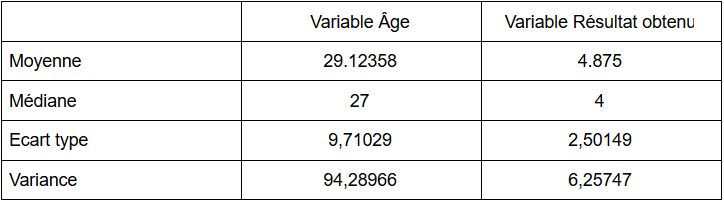
\includegraphics[width=0.7\textwidth]{./Images/2}
	\caption{Tableau représentant les statistiques sur les variables quantitatives étudiées}
\end{figure}

\section{Autisme}
	Lors de notre étude, notre but est d’expliquer cette variable, de savoir s’il est possible de la prévoir. 0 indique que l’individu n’est pas atteint d’un trouble du spectre autistique tandis que 1 indique que l’individu étudié est atteint de cet handicap.\\
	
\begin{figure}[!ht]
	\center
	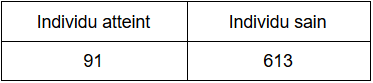
\includegraphics[width=0.4\textwidth]{./Images/3}
	\caption{Tableau de répartition des individus selon l'autisme}
\end{figure}\vspace{0.1cm}

On peut remarquer ici que cet handicap est plutôt bien représenté dans un échantillon de taille suffisamment importante puisque 13\% de l’échantillon présente un trouble du comportement autistique.
\section{Âge}
	L’individu le plus jeune a 17 ans tandis que le plus âgé a 64 ans.
Voici un diagramme indiquant la répartition, selon l’âge, des individus atteint d’un trouble du spectre autistique.\\

\begin{figure}[!ht]
	\center
	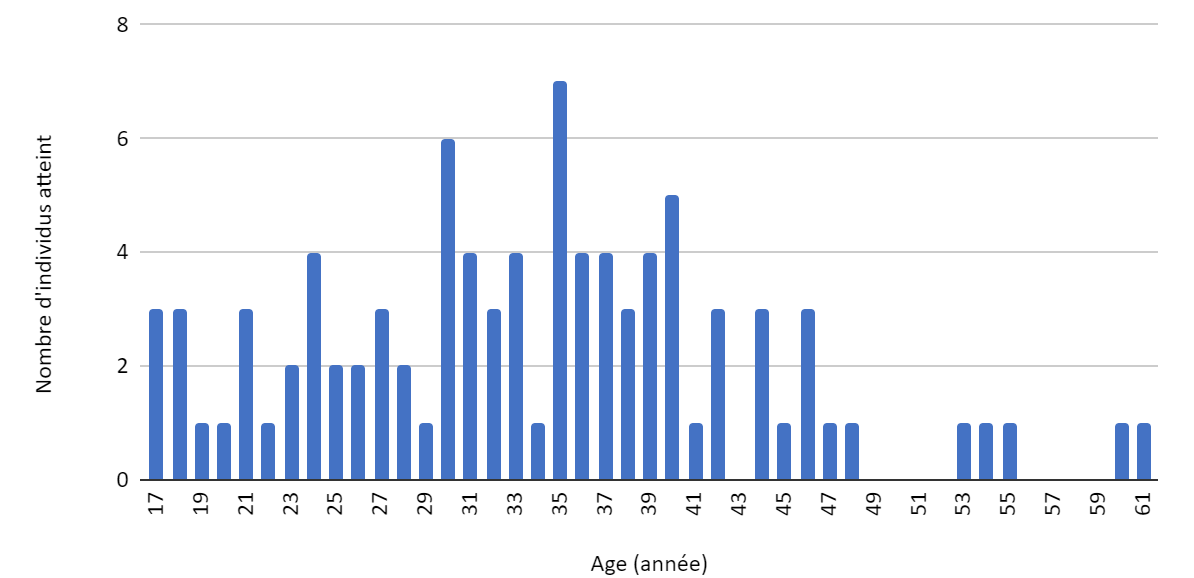
\includegraphics[width=0.7\textwidth]{./Images/4'}
	\caption{Graphique représentant le nombre d'individus atteints en fonction de l'âge}
\end{figure}\vspace{0.2cm}

	On remarque sur ce diagramme que la tranche d’âge la plus touchée est celle des individus ayant une trentaine d’années ainsi que les plus jeunes. On remarque peu de cas à partir de 50 ans, on peut donc se demander si la durée de vie est raccourcie pour les personnes atteintes de ce syndrome.\\
	
\begin{figure}[!ht]
	\center
	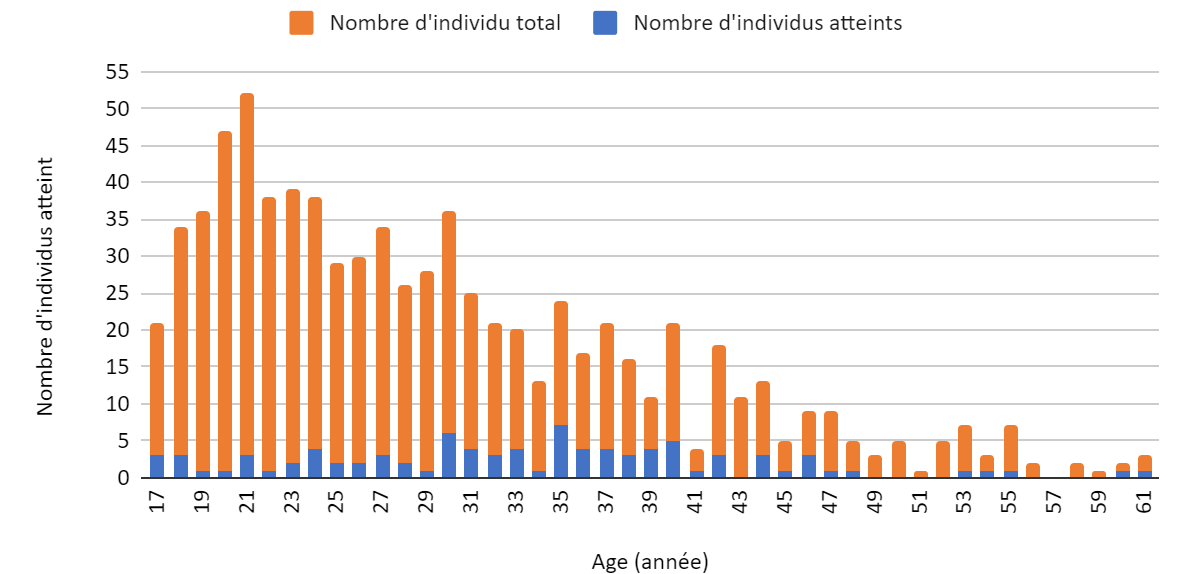
\includegraphics[width=0.8\textwidth]{./Images/5'}
	\caption{Graphique représentant le nombre d'individus atteints et total selon leur age}
\end{figure}\vspace{0.4cm}

	Toutefois, ce diagramme indique que la tranche d’âge à partir de 48 ans est tout simplement très peu représentée dans l’échantillon d’où le manque de données sur ces individus. On notera que deux individus n’ont pas indiqué leur âge, cependant ce ne sont pas des individus atteints cela ne pose donc pas énormément de problème.

Ci-dessous, nous avons représenté la boite à moustache de la variable âge afin de visualiser la médiane ainsi que la distance interquartile. Les valeurs supérieure	s à 56 ans sont hors épure, ces points sont ainsi suspects (très peu de personnes âgées parmis nos individus).\\

\begin{figure}[!ht]
	\center
	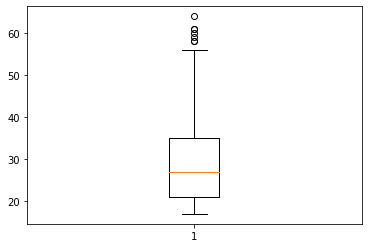
\includegraphics[width=0.7\textwidth]{./Images/6}
	\caption{Boîte à moustache de la varaible Âge}
\end{figure}\vspace{0.1cm}

	La répartition de notre échantillon est en grande majorité sur des personnes ayant entre 20 et 40 ans, ce que nous confirme ce schéma.

\section{Genre}
Le meilleur moyen de présenter cette variable est là encore un tableau.\\

\begin{figure}[!ht]
	\center
	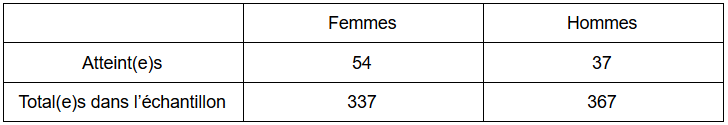
\includegraphics[width=0.7\textwidth]{./Images/7}
	\caption{Tableau du nombre d'individus atteints et total selon le sexe}
\end{figure}\vspace{0.1cm}

	Les femmes semblent plus touchées par ce syndrome puisqu’on relève : 16\% des femmes sont atteintes contre 10\% chez les hommes. Dans cet échantillon, parmi les 91 individus présentant ce trouble, presque un tiers sont des femmes.

    En effet, on peut évaluer le rapport entre les individus atteints et non atteints pour chacun des deux genres :

\begin{itemize}
	\item Femmes : $\frac{54}{283}=0,19081$
	\item Hommes : $\frac{37}{337}=0,10979$
\end{itemize}

	Le rapport pour les femmes étant bien supérieur, la gente féminine semble donc plus vulnérable face à ce syndrome.

\section{Né avec la jaunisse}
	Sur l’ensemble des 704 individus, seulement 69 d’entre eux sont nés avec la jaunisse, soit un peu moins de 10\%. Or dans l’échantillon des 91 individus atteints, on relève 20 personnes nées avec la jaunisse soit 21,92\% contre 49 cas sur 564 parmis les individus sains soit environ 8\%. \\

\begin{figure}[!ht]
	\center
	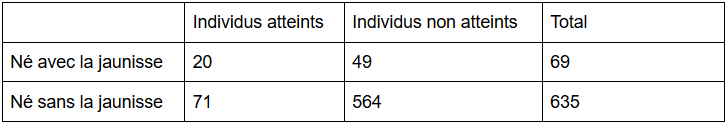
\includegraphics[width=0.7\textwidth]{./Images/8}
	\caption{Tableau de contingence entre Né avec la jaunisse et Autisme}
\end{figure}\vspace{0.1cm}

	Même si parmi les individus atteints la proportion de Né avec la jaunisse est plus importante que parmi les individus non atteints, il semblerait à priori que cette variable n’est pas réellement décisive sur le fait que l’individu présente le trouble ou non.

\section{A1\_score à A10\_score}
	Tout d’abord, calculons la moyenne des scores obtenus pour chacune de ces questions. Nous rappelons ici que la valeur 0 indique que l’individu est d’accord (‘oui’)  avec la proposition A ainsi 1 traduit son désaccord (‘non’).\\

\begin{figure}[H]
	\center
	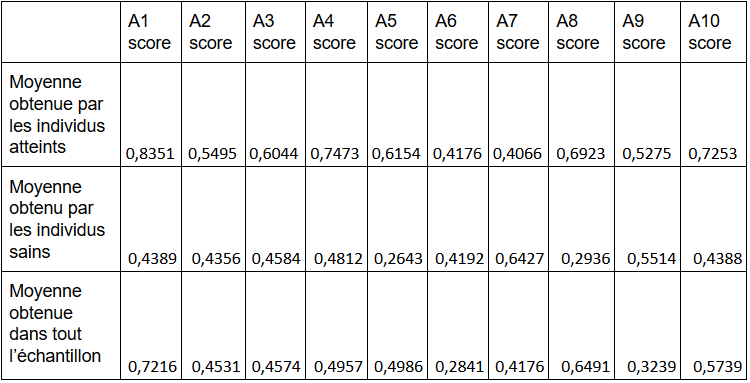
\includegraphics[width=0.7\textwidth]{./Images/9}
	\caption{Moyenne des scores obtenus sur les 10 questions des individus atteints et non atteints}
\end{figure}\vspace{0.1cm}

	Ici, un diagramme sera plus représentatif afin de comparer les moyennes obtenues par les individus sains et celles obtenues par les individus atteints du trouble.\\

\begin{figure}[H]
	\center
	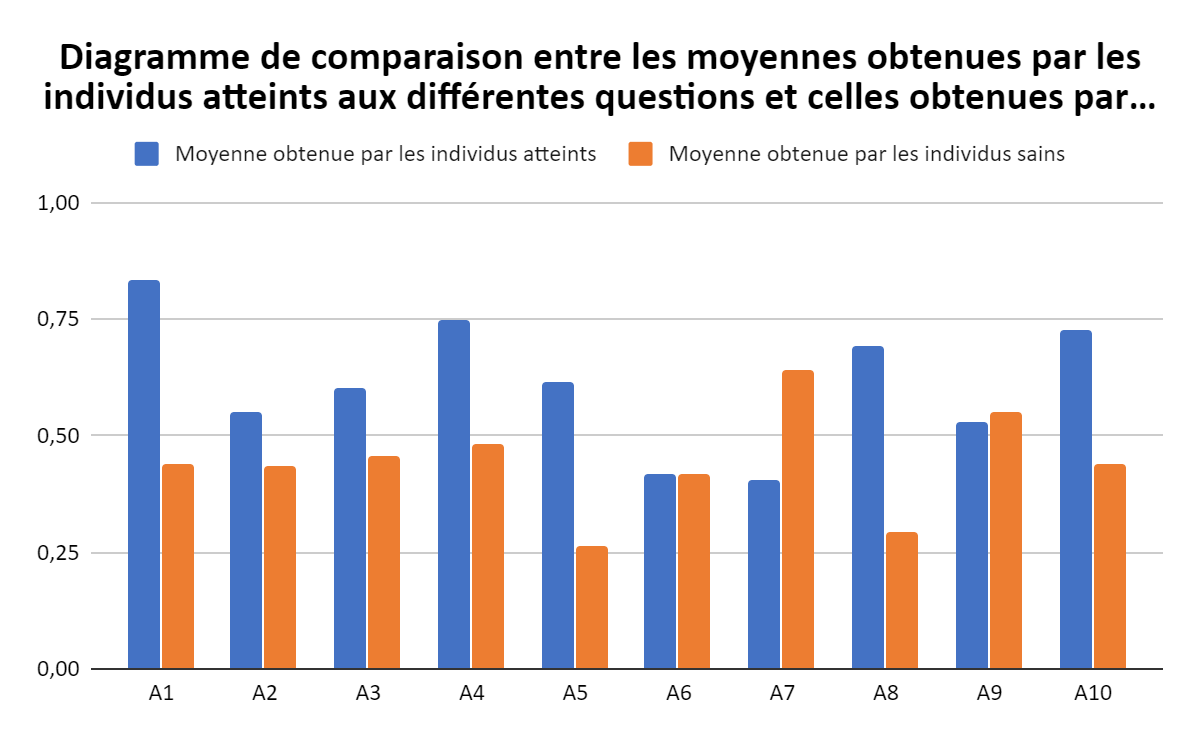
\includegraphics[width=0.7\textwidth]{./Images/10}
	\caption{Diagramme comparant les moyennes des scores des individus atteints et non atteints}
\end{figure}\vspace{0.1cm}

	Grâce à ce diagramme, on remarque que certaines réponses aux questions semblent être décisives quant à la présence du trouble chez un individu ou non. En effet, un individu atteint du trouble du spectre autistique :

\begin{itemize}
	\item remarquera moins souvent de petits bruits que d’autres ne remarquent pas
	\item se concentrera davantage sur les détails que sur l’image
	\item ne trouvera pas facile d’entreprendre deux choses à la fois
	\item aura du mal à revenir à ce qu’il faisait en cas d’interruption
	\item aura des difficultés à lire entre les lignes quand on lui parle
	\item rencontrera de plus grandes difficultés pour déterminer les intentions  des personnages d’une histoire
	\item ne rassemblera pas particulièrement d’informations sur des catégories d’objets
	\item ne trouvera pas difficile de comprendre les intentions des gens
\end{itemize}

\section{Score obtenu}
	En moyenne, un individu atteint de l’autisme obtient une note d’environ 6,12 tandis qu’un individu sain obtiendra plutôt un 4,68 c’est à dire une majorité de “oui” aux questions A1 à A10.
	
\section{Appli détecte autisme}
L’application a détecté, en tout, 189 cas d’autisme parmi les 704 individus de l’échantillon. Parmi eux on relève 146 individus sains et donc seulement 43 individus réellement atteints du trouble du spectre autistique. parmi les 91 individus réellement atteints, l’application n’en a détecté que 47,3\% d’entre eux, soit moins de la moitié. L’application semble ainsi à premier abord très peu fiable.


\section{Déjà utilisé l'application}
Parmi l’ensemble des individus, seulement 12 avaient déjà utilisé l’application, et seulement 2 sont atteints parmi ces derniers. Cette variable est inutile pour prévoir si oui ou non un individu est atteint ou pas.
\section{Pays de résidence}
Grâce à des calculs sur Colab Notebook, nous avons pu obtenir les pourcentages de répartition des individus par pays de résidence. Nous avons ainsi pu remarquer que 16,1\% vivent aux Etats Unis, 11,6\% aux Emirats Arabes, 11,5\% en Inde ou encore en Nouvelle Zélande, 10,9\% en Grande Bretagne et seulement 1,6\% en France.\\

\begin{figure}[H]
	\center
	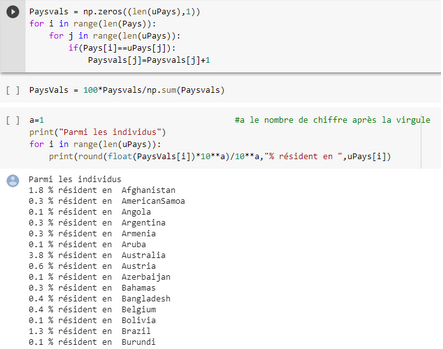
\includegraphics[width=0.6\textwidth]{./Images/11}
	\caption{Capture de \textit{Colab} désignant la répartition des individus selon leur pays de résidence}
\end{figure}\vspace{0.1cm}

	Nous avons ensuite trouvé intéressant de calculer le pourcentage de répartition des individus par pays de résidence mais cette fois en sachant qu’ils sont atteints du trouble du spectre autistique, c’est à dire que nous avons classé les 91 individus atteints en fonction de leur lieu de vie. Ainsi, parmi les 91 cas, 25,3\% vivent aux Etats Unis, 18,7\% en Grande Bretagne, 3,3\% aux Emirats Arabes, 2,2\% en Inde et enfin 3,3\% en France.\\
	
	Ces chiffres n’étant pas très parlant, nous allons donc calculer les rapports entre ceux atteints et ceux qui résident au sein des Pays afin que ces chiffres nous soient plus significatifs :

\begin{itemize}
	\item Etats-Unis : $\frac{0.253*91}{0,161*704}=0,203$
	\item Grande Bretagne : $\frac{0.187*91}{0.109*704}=0,222$
	\item Emirats Arabes : $\frac{0.033*91}{0,116*704}=0,037$
	\item France : $\frac{0.033*91}{0,016*704}=0,267$
\end{itemize}\vspace{0.3cm}

	Il semblerait ici que certains pays soient plus touchés que d’autres par cet handicap, par exemple les Emirats Arabes sont six fois moins touchés que la Grande Bretagne alors qu’ils sont plus représentés dans l’échantillon. En effet, si on calcule les effectifs pour chaque pays, 3,7\% des individus de l’échantillon vivants aux Emirats Arabes sont atteints contre 22,1\% en Grande Bretagne. Cette variable ne semble pas très significative de la détection d’un cas d’autisme.

\section{Ethnique}
	Nous nous sommes ensuite intéressés à la variable qualitative Ethnique. De même que pour la variable Pays de résidence nous avons dressé la répartition des individus en fonction de leur Ethnique.\\

	Parmi les individus :
\begin{itemize}
	\item 17.5 \% ont une ethnique  Asian
	\item 6.1 \% ont une ethnique  Black
	\item 1.8 \% ont une ethnique  Hispanic
	\item 2.8 \% ont une ethnique  Latino
	\item 13.1 \% ont une ethnique  Middle Eastern '
	\item 4.3 \% ont une ethnique  Others
	\item 1.7 \% ont une ethnique  Pasifika
	\item 5.1 \% ont une ethnique  South Asian'
	\item 0.9 \% ont une ethnique  Turkish
	\item 33.1 \% ont une ethnique  White-European
	\item 13.5 \% ont une ethnique  inconnue
	\item 0.1 \% ont une ethnique  others
\end{itemize}\vspace{0.3cm}

	Nous remarquons donc une grande majorité d’Européens dans notre échantillon et très peu de Turcs, Hispanics ou encore de Latinos.
	
	Ensuite nous avons voulu savoir qu’elle était alors, en terme d'individus atteints du trouble d’autisme, la nouvelle répartition.\\
	
	Parmi les individus atteints :
\begin{itemize}
	\item 5.5 \% ont une ethnique  Asian
	\item 5.5 \% ont une ethnique  Black
	\item 1.1 \% ont une ethnique  Hispanic
	\item 8.8 \% ont une ethnique  Latino
	\item 9.9 \% ont une ethnique  Middle Eastern '
	\item 2.2 \% ont une ethnique  Others
	\item 2.2 \% ont une ethnique  Pasifika
	\item 2.2 \% ont une ethnique  South Asian'
	\item 1.1 \% ont une ethnique  Turkish
	\item 54.9 \% ont une ethnique  White-European
	\item 6.6 \% ont une ethnique  inconnue
\end{itemize}\vspace{0.3cm}

	On remarque ici une grosse concentration sur l’Ethnique White-European parmi ceux atteints, à se demander si le fait de faire partie de cette Ethnique influe sur le fait d’être atteint.
	
	Pour avoir une idée plus précise, nous nous sommes intéressés à chaque ethnique pour ainsi mieux mettre en avant les plus touchées. Grâce à Colab nous obtenons les proportions suivantes :\\
	
\begin{itemize}[label=$\blacksquare$]
	\item 4.1 \% ayant une ethnique  Asian  sont atteints
	\item 11.6 \% ayant une ethnique  Black  sont atteints
	\item 7.7 \% ayant une ethnique  Hispanic  sont atteints
	\item 40.0 \% ayant une ethnique  Latino  sont atteints
	\item 9.8 \% ayant une ethnique  Middle Eastern '  sont atteints
	\item 6.7 \% ayant une ethnique  Others  sont atteints
	\item 16.7 \% ayant une ethnique  Pasifika  sont atteints
	\item 5.6 \% ayant une ethnique  South Asian'  sont atteints
	\item 16.7 \% ayant une ethnique  Turkish  sont atteints
	\item 21.5 \% ayant une ethnique  White-European  sont atteints
	\item 6.3 \% ayant une ethnique  inconnu  sont atteints
\end{itemize}\vspace{0.3cm}

Avec cette étude, les Latinos semblent être les plus vulnérables face à cet handicap contrairement à l’Asie du Sud, même si l’échantillon de Latinos est assez faible pour conclure. Les Européens restent cependant les deuxièmes plus touchés avec 21,5\%, nous verrons par la suite si ce facteur est vraiment significatif.

\section{Parenté avec l'individu}
	Enfin, nous avons analysé de la même façon la variable “Parenté avec l’individu réalisant le test” et avons remarqué que :\\
	
	Parmi les individus :
\begin{itemize}[label=\textbullet]
	\item 13.5 \% ont une Parenté  inconnue 
	\item 0.6 \% ont une Parenté  Health care professional' (=professionnel 		de la santé)
	\item 0.7 \% ont une Parenté  Others
	\item 7.1 \% ont une Parenté  Parent
	\item 4.0 \% ont une Parenté  Relative (=Ami)
	\item 74.1 \% ont une Parenté  Self (=Soi même)
\end{itemize}\vspace{0.3cm}

\pagebreak

	De plus,
\begin{itemize}
	\item 6.3 \% ayant une Parenté Inconnue  sont atteints
	\item 25.0 \% ayant une Parenté  Health care professional  sont atteints
	\item 20.0 \% ayant une Parenté  Others  sont atteints
	\item 26.0 \% ayant une Parente  Parent  sont atteints
	\item 21.4 \% ayant une Parenté  Relative  sont atteints
	\item 12.3 \% ayant une Parenté  Self  sont atteints
\end{itemize}\vspace{0.3cm}

	La répartition des cas est plus ou moins répartie de la même manière selon les différents liens de parenté. On remarque cependant un taux un peu plus faible pour les individus atteints lorsqu’on possède une parenté Self. La variable Parenté avec l'individu semblerait alors très peu significative pour reconnaître un cas d’autisme ou non.

\chapter{Analyse en Composantes Principales (ACP)}
	Pour comprendre les liens entre les différentes variables et les individus nous avons réalisé une ACP. Les variables étudiées ici sont uniquement les variables quantitatives.
	
\section{Centrer et réduire}
Nous avons commencé par centrer et réduire dans le but de pouvoir comparer des choses comparables sans effet de “taille” notamment pour l’âge puisque le reste des variables sont principalement des variables binaires. On obtient alors la matrice symétrique de Covariance-Variance suivante :\\

\begin{figure}[H]
	\center
	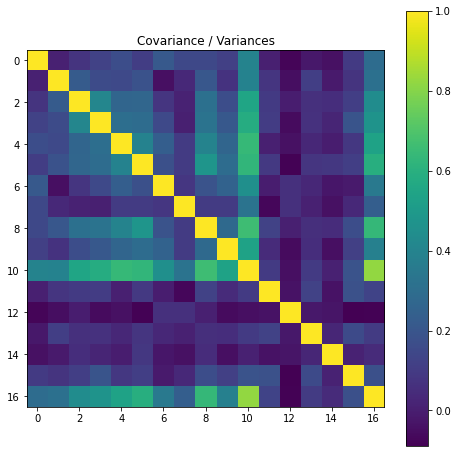
\includegraphics[width=0.7\textwidth]{./Images/12}
	\caption{Matrice de covariance-variance des variables}
\end{figure}\vspace{0.1cm}

	On retrouve bien que la 11ème variable (n°10 sur le schéma) ,qui représente la note totale obtenue aux réponses aux 10 premières questions, dépend bien des 10 premières variables qui sont elles-mêmes ces réponses. En effet cette 11ème variable est la somme des 10 premières variables binaires.
De plus, on peut noter que la 17ème variable, qui n’est autre que la variable qui indique si l’application considère l’individu présente ou non ce trouble, présente une forte dépendance de la 11ème variable c’est à dire la note totale. En effet, si cette somme est supérieur à 7, l’algorithme conclut que l’individu est atteint de cet handicap. Implicitement, la variable indiquant la réponse de l’application dépend ainsi uniquement des 10 premières variables qui sont les réponses aux questions A1 à A10.

\section{Valeurs propres}
    Nous avons ensuite calculé les valeurs propres et vecteurs propres associés afin de déduire les axes principaux les plus importants. Nous avons obtenu la matrice de vecteurs propres suivante :\\

\begin{figure}[H]
	\center
	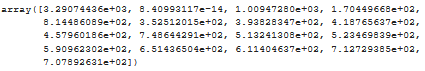
\includegraphics[width=0.7\textwidth]{./Images/13}
	\caption{Matrice des vecteurs propres originale}
\end{figure}\vspace{0.1cm}

	En réarrangeant les valeurs de la matrice afin d’avoir les plus significatives en premières on a obtenu la matrice suivante :\\
	
\begin{figure}[H]
	\center
	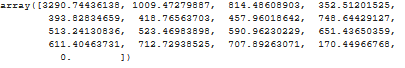
\includegraphics[width=0.7\textwidth]{./Images/14}
	\caption{Matrice des vecteurs propres arrangée}
\end{figure}\vspace{0.1cm}

	On obtient alors :

\begin{figure}[H]
	\center
	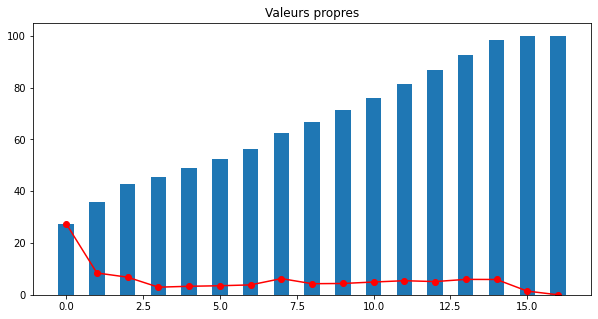
\includegraphics[width=0.7\textwidth]{./Images/15}
	\caption{Diagramme bâton des vecteurs propres}
\end{figure}\vspace{0.1cm}

	Les trois premières valeurs représentent ainsi 43\% de l’information.
	
\section{Projection selon plusieurs axes}
Nous avons donc décidé de projeter dans un premier temps le nuage de points représentant les individus sur les axes des deux principaux facteurs. On obtient alors le nuage de points suivant :\\

\begin{figure}[H]
	\center
	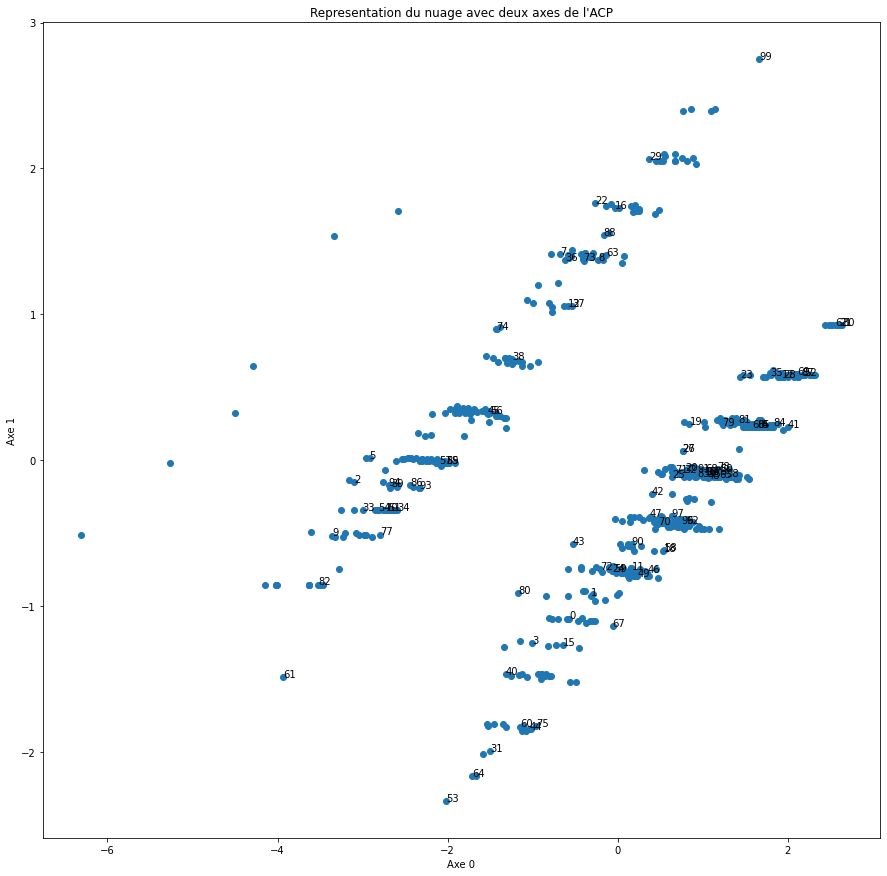
\includegraphics[width=0.53\textwidth]{./Images/16}
	\caption{Projection des individus sur les deux axes principaux}
\end{figure}\vspace{0.1cm}

	Enfin, en projetant les variables dans le plan des deux principaux facteurs,on a obtenu la représentation suivante :\\


\begin{figure}[H]
    \begin{minipage}[c]{.46\linewidth}
        \centering
        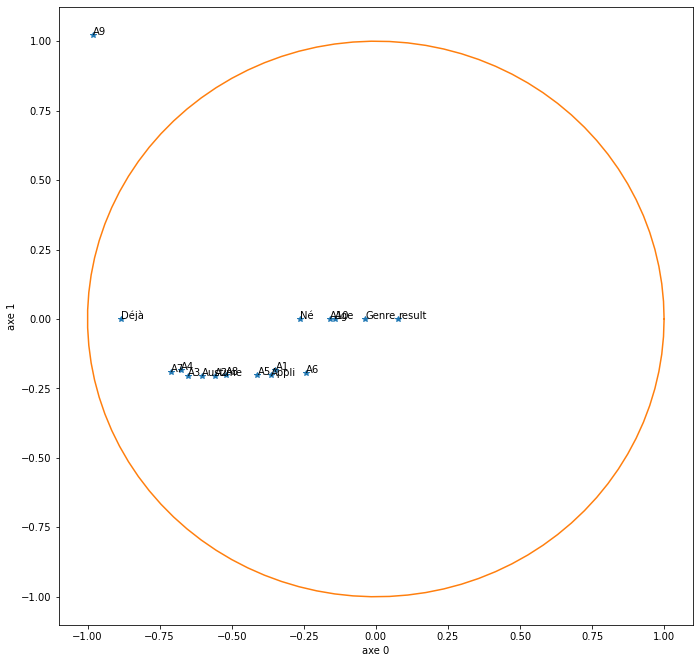
\includegraphics[width=1\textwidth]{./Images/17}
        \caption{Projection des variables sur les deux axes principaux}
    \end{minipage}
    \hfill%
    \begin{minipage}[c]{.46\linewidth}
        \centering
        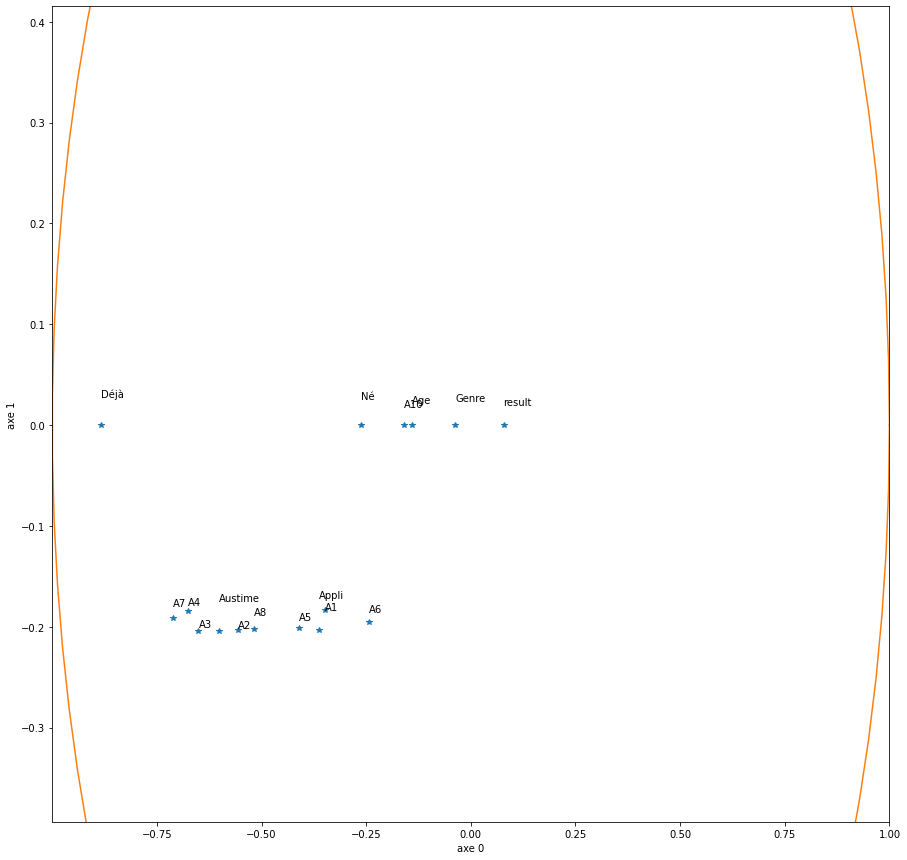
\includegraphics[width=1\textwidth]{./Images/18}
        \caption{Projection zoomée des variables sur les deux axes principaux}
    \end{minipage}
\end{figure}\vspace{0.1cm}

\pagebreak

	On en a donc déduit que la variable A9 étant hors du cercle de corrélation, n’était pas réellement significative tandis que les variables allant de A1 à A8 ainsi que la réponse de l’appli, formant un nuage de points avec la variable autisme présente un lien fort entre elles.
	
    Afin de confirmer cela, nous avons réalisé la projection des variables dans le plan définit par le premier et le troisième principal facteur. Nous avons alors obtenu la répartition du nuage de points suivant : \\
    
\begin{figure}[H]
    \begin{minipage}[c]{.46\linewidth}
        \centering
        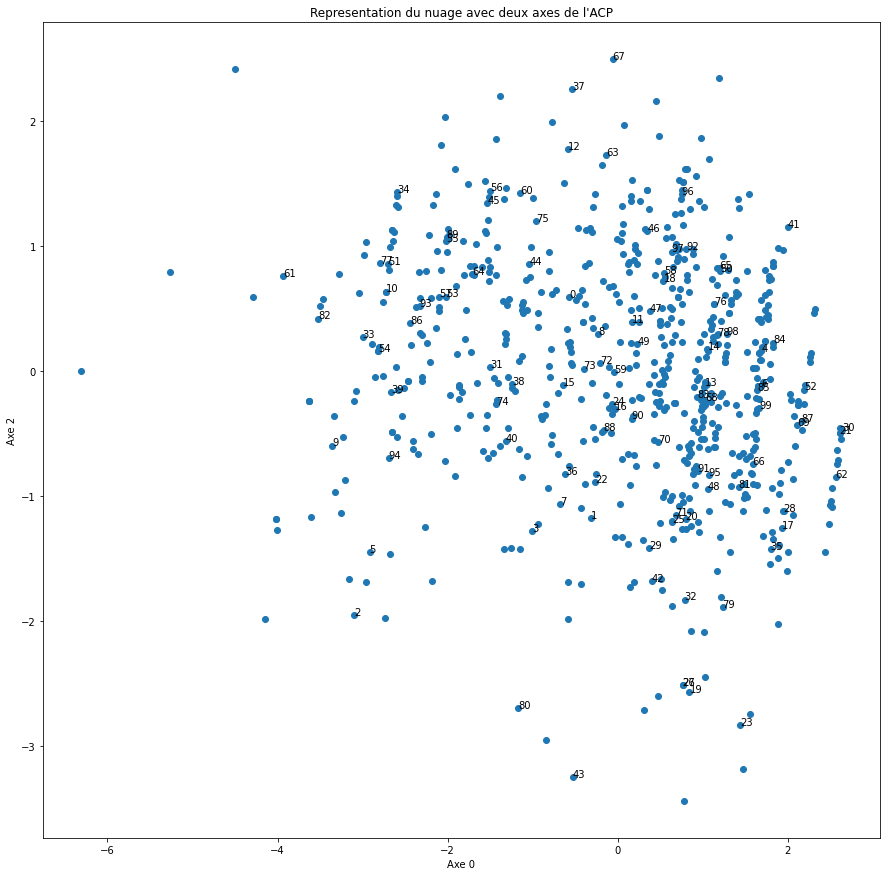
\includegraphics[width=1\textwidth]{./Images/19}
        \caption{Projection des individus sur le premier et troisième axe}
    \end{minipage}
    \hfill%
    \begin{minipage}[c]{.46\linewidth}
        \centering
        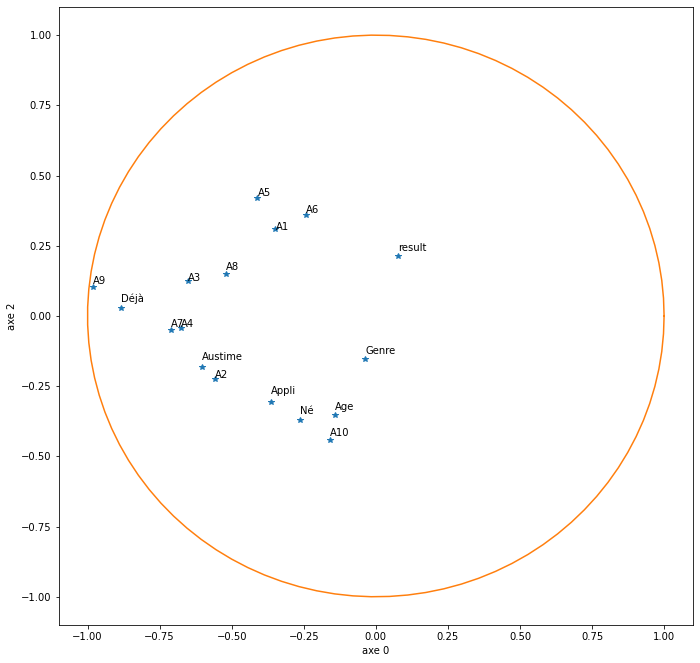
\includegraphics[width=1\textwidth]{./Images/20}
        \caption{Projection des variables sur le premier et troisième axe}
    \end{minipage}
\end{figure}\vspace{0.1cm}

Là encore, on remarque l’éloignement de la variable A9 par rapport à celle autisme. Or les variables A2, A4 et A7 sont très proches de la variable autisme et semblent donc avoir une importance plus déterminante que les autres.

\chapter{Régression linéaire multiple}

Afin d’analyser la possibilité de prédire l’autisme d’un individu ou non en fonction des réponses aux 10 questions A1 à A10, nous avons utilisé la régression linéaire. En effet, l’application annonce que l’individu est autiste uniquement si le résultat obtenu à ces questions est supérieur ou égal à 7. Si cela est possible par hypothèse, nous devrions alors obtenir un indice de qualité de régression (R2) proche de 1 signifiant ainsi que le modèle est bon.
    En choisissant $y = 1$ si l’individu est autiste, 0 s’il ne l’est pas, et $x1=A1, x2=A2…,x10=A10$. Soit $X=[x1,x2,...,x10],$  nous obtenons $Y=aX$ avec a la matrice de régression :

\begin{figure}[H]
	\center
	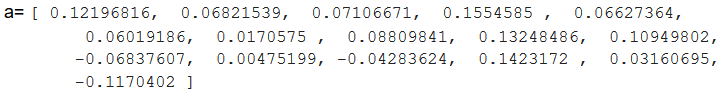
\includegraphics[width=0.7\textwidth]{./Images/a}
\end{figure}\vspace{0.1cm}

La représentation des résidus de la régression $e = y-Xa$ est la suivante :

\begin{figure}[H]
	\center
	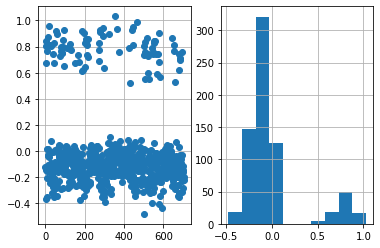
\includegraphics[width=0.7\textwidth]{./Images/21}
	\caption{Nuage de point et diagramme des résidus}
\end{figure}\vspace{0.1cm}

Ainsi on obtient un R2=0,10538 et le schéma de la régression suivant où les points rouges représentent $y$ et les points verts sont $z=Xa$ c’est à dire la prédiction de la variable autisme grâce à cette régression linéaire :

\pagebreak

\begin{figure}[H]
	\center
	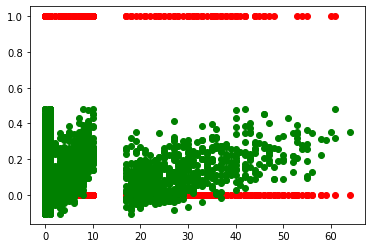
\includegraphics[width=0.7\textwidth]{./Images/22}
	\caption{Résultat de la régression linéaire multiple}
\end{figure}\vspace{0.1cm}

On remarque donc que le R2 est proche de 0 c’est à dire que le modèle de régression est mauvais donc que la variable autisme ne peut pas être prédit à l’aide uniquement des réponses aux questions A1 à A10. Là encore, on en déduit que l’algorithme de détermination d’un cas d’autisme sur lequel repose l’application ASD Tests n’est pas fiable.



\chapter{Régression logistique}
Notre régression linéaire n’ayant pas été satisfaisante, nous avons tenté de réaliser une régression logistique avec l’aide de notre chargé de TD, Cyprien Ruffino. Ce modèle semble plus adapté à nos données. En effet, en posant $p$ la probabilité que notre variable autisme (ici y) vaut 1, on pose alors la régression linéaire comme :

$$ \ln\frac{p}{1-p}=\beta+\sum_{i=1}^{p}\alpha_{p}x_{p} $$

Ainsi il existe une relation entre $X$ (la matrice des variables $x0\dots xn$) et le logit de $y$ telle que :

$$y=\frac{1}{1+\exp(-z)}$$
$$z=\beta+\sum_{i=1}^{p}\alpha_{p}x_{p} $$

La représentation graphique obtenue est la suivante : \\

\begin{figure}[H]
	\center
	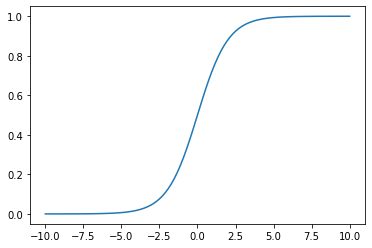
\includegraphics[width=0.7\textwidth]{./Images/23}
	\caption{Logit de la régression logistique}
\end{figure}\vspace{0.1cm}

On notera que cette représentation correspond bien à une représentation de régression logistique. Nous avons ensuite procédé à une sélection de variables grâce à la fonction SelectFromModel. Cette dernière a affirmé que les six variables avec les plus grands coefficients sont les variables Âge, Né avec la jaunisse, le Résultat obtenu, le Genre ainsi que les réponses aux questions A4 et A7. Lorsque l’on évalue le modèle, on obtient une précision de 0,87, ce qui est proche de 1. Ainsi cette valeur permet d’admettre raisonnablement que le modèle est bon.

\chapter{Tableaux de contingence et test du chi2}
Dans le but de juger de la dépendance entre les variables (que la régression logistique a jugé importante) et la variable autisme, nous avons réalisé des tableaux de contingence, évalué les distances du chi2 obtenues pour chacune des variables associées à la variable autisme, et avons calculé la p-valeur associée à chacune d’entre elles. On a également étudié ces estimateurs pour la variable A2 que notre ACP avait considéré comme proche de la variable autisme. \\

\section{Effectifs normaux}

Voici les tableaux de contingence des observations obtenues :\vspace{0.5cm}

\begin{figure}[H]
	\center
	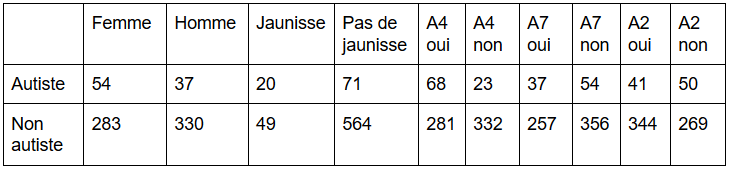
\includegraphics[width=0.7\textwidth]{./Images/24}
	\caption{Tableau de contingence entre plusieurs variables}
\end{figure}\vspace{0.5cm}

\begin{figure}[H]
	\center
	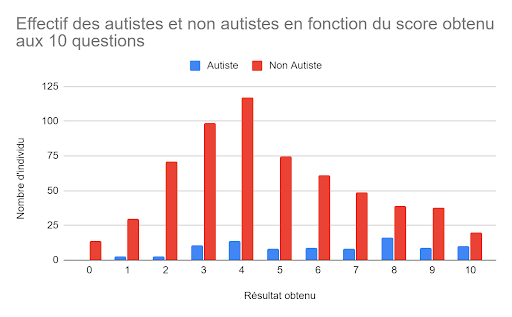
\includegraphics[width=0.7\textwidth]{./Images/25}
	\caption{Graphique représentant la répartition des individus selon leurs réponses aux questions}
\end{figure}\vspace{0.5cm}

\begin{figure}[H]
	\center
	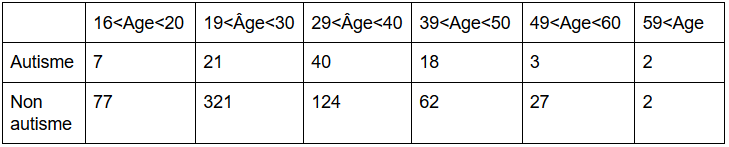
\includegraphics[width=0.7\textwidth]{./Images/26}
	\caption{Tableau de contingence entre Âge et Autisme}
\end{figure}\vspace{0.6cm}

\section{Effectifs théoriques}
Voici ensuite les tableaux de contingence des effectifs théoriques :\\

\begin{figure}[H]
	\center
	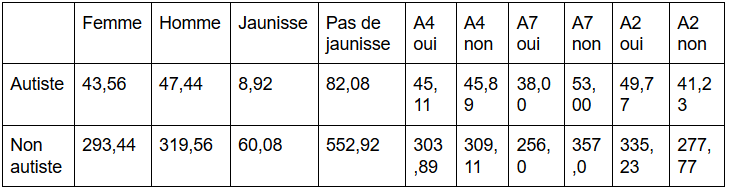
\includegraphics[width=0.7\textwidth]{./Images/27}
	\caption{Tableau de contingence des effectifs théoriques entre plusieurs variables}
\end{figure}\vspace{0.1cm}

\begin{figure}[H]
	\center
	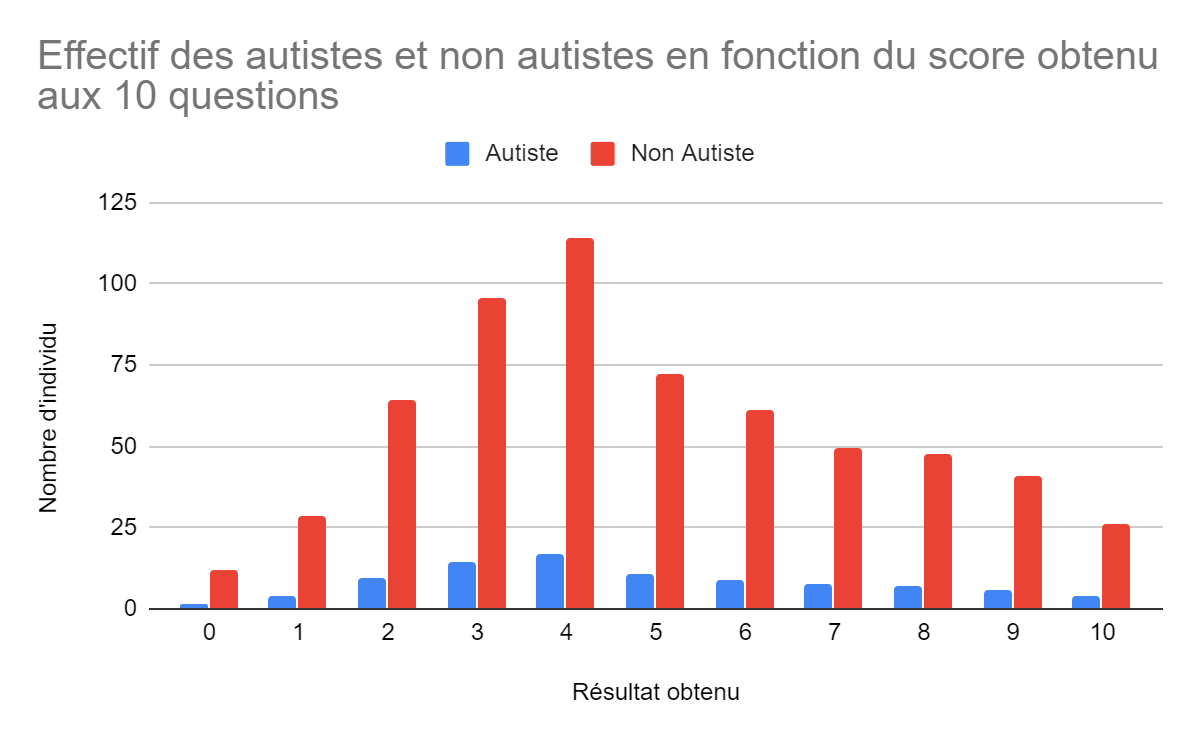
\includegraphics[width=0.7\textwidth]{./Images/28}
	\caption{Graphique représentant la répartition théorique des individus selon leurs réponses aux questions}
\end{figure}\vspace{0.1cm}

\begin{figure}[H]
	\center
	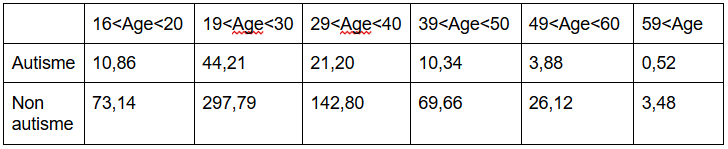
\includegraphics[width=0.7\textwidth]{./Images/29}
	\caption{Tableau de contingence des effectifs théoriques entre Âge et 			Autisme}
\end{figure}\vspace{0.1cm}

\section{\boldmath$\displaystyle\chi^2 $\unboldmath et p-valeurs}
On obtient alors les valeurs de chi2 et les p-valeurs entre la variable et les différentes variables suivantes :\\

\begin{figure}[H]
	\center
	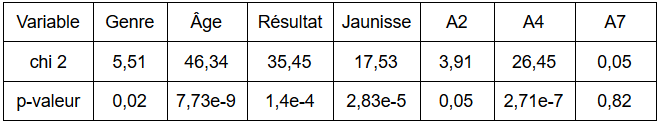
\includegraphics[width=0.7\textwidth]{./Images/30}
	\caption{Tableau avec le $\chi^2$ et la p-valeur des variables suivantes}
\end{figure}\vspace{0.1cm}

En étudiant les p-valeurs et en fixant l’erreur de première espèce acceptable à 0,05, on peut raisonnablement affirmer que la variable autisme dépend de sa réponse aux questions A2 et A7.

\chapter*{Conclusion}
\addcontentsline{toc}{chapter}{Conclusion}

En étudiant l’algorithme de décision de l’application ASD Tests qui permet d’identifier un trouble du spectre autistique chez un individu, ainsi que l’ACP obtenue lors de l’étude de la base de données de l’application, nous avons pu justifier raisonnablement que celle-ci n’était pas fiable. En effet, elle présente un nombre conséquent d’erreurs et l’ACP a justifié cela en mettant en avant notamment le fait que la variable Autiste était peu dépendante du score obtenu, alors que l’application affirme que l’individu est atteint si ce score est supérieur à 7.\\

    Toutefois, grâce aux données que l’application enregistre sur l’individu étudié, le programme peut être amélioré en modifiant l’importance de certaines variables. Ceci a été prouvé par la régression logistique. La régression a estimé les variables Genre, Âge, Né avec la jaunisse, Résultat ainsi que les réponses aux questions A4 (S’il y a une interruption je peux très facilement revenir à ce que je faisais) et A7 (Quand je lis une histoire je trouve difficile de déterminer les intentions des personnages) comme plus importantes. Le test du chi2 et l’étude des p-valeurs nous ont permis d’étudier la dépendance entre la variable Autiste et chacune de ces variables définies comme caractéristiques d’un autiste par la régression. L’individu type semble rencontrer des difficultés à déterminer l’intention des personnages quand il lit une histoire puisque cette hypothèse a été validée par l’ACP, la régression logistique ainsi que le test du chi2 ce qui est très révélateur. En ce qui concerne les autres variables, les différents estimateurs ne permettent pas de conclure suite à des contradictions.\\

    Du fait de la liberté du choix du thème de notre projet, nous avons pu travailler sur un sujet qui nous plaît réellement, ce qui nous a facilité l’envie d’approfondir certaines notions. Restituer les connaissances vu en cours afin de les adapter de manière concrète dans notre projet fut très bénéfique dans l’apprentissage et la compréhension de la M8. 
Ce projet nous a ainsi permis d'étudier une base de données afin de la comprendre et de l'expliquer scientifiquement.

\listoffigures

\iffalse
\chapter*{Bibliographie}
\addcontentsline{toc}{chapter}{Bibliographie}

Dans le fichier bibliohraphie.bib, vous mettez vos références, par exemple les
 noms des livres, article, siteweb, cours ... que vous avez utilisé pour faire
 ce travail.
 \fi

\chapter*{Annexes}
\addcontentsline{toc}{chapter}{Annexes}
Voici un aperçu de nos données :\vspace{1cm}

\begin{figure}[H]
	\centering
	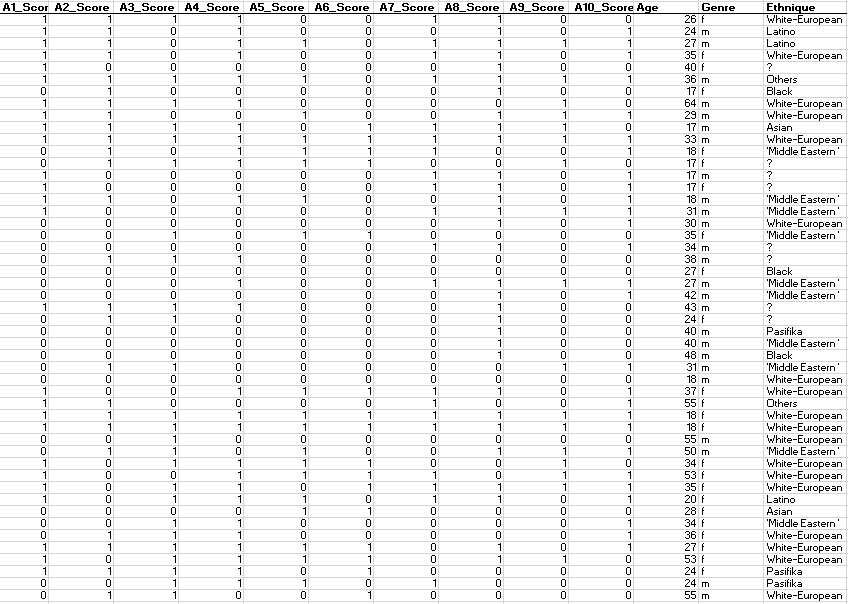
\includegraphics[height=0.5\textheight]{./Images/1}\vspace{0.4cm}
	%\caption*{Extrait des données de notre échantillon\protect\refstepcounter{footnote}\protect\footnotemark[\thefootnote]}
	Extrait des données de notre échantillon\footnote[1]{source1}
\end{figure}\vspace{0.5cm}

\begin{minipage}{1\textheight}
\vspace{3.9cm}
\end{minipage}

\footnotetext[1]{Données obtenues sur le \textcolor{blue}{\href{https://archive.ics.uci.edu/ml/datasets/Autism+Screening+Adult}{site}} de l’UCI}

\begin{figure}[H]
	\centering
	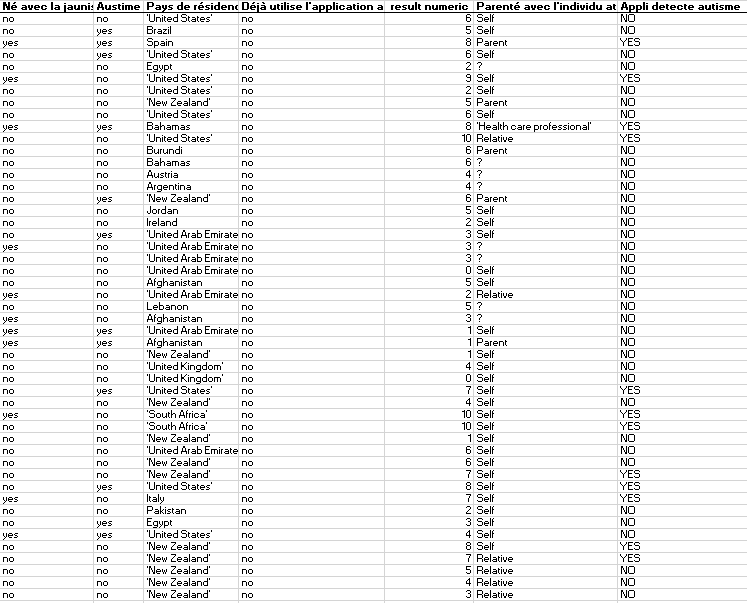
\includegraphics[height=0.6\textheight]{./Images/1'}\vspace{0.4cm}
	%\caption*{Extrait des données de notre échantillon\protect\refstepcounter{footnote}\protect\footnotemark[\thefootnote]}
	Extrait des données de notre échantillon\footnote[1]{source1}
\end{figure}\vspace{0.5cm}

\footnotetext[1]{Données obtenues sur le \textcolor{blue}{\href{https://archive.ics.uci.edu/ml/datasets/Autism+Screening+Adult}{site}} de l’UCI}


%\captionsetup[figure]{list=no}

\end{document}
